%iffalse
\let\negmedspace\undefined
\let\negthickspace\undefined
\documentclass[journal,12pt,onecolumn]{IEEEtran}
\usepackage{cite}
\usepackage{amsmath,amssymb,amsfonts,amsthm}
\usepackage{algorithmic}
\usepackage{graphicx}
\usepackage{textcomp}
\usepackage{xcolor}
\usepackage{txfonts}
\usepackage{listings}
\usepackage{tikz}
\usepackage{circuitikz}
\usetikzlibrary{patterns}
\usetikzlibrary{arrows.meta}
\usetikzlibrary{angles}
\usetikzlibrary{patterns}
\usetikzlibrary{intersections}
\usepackage{enumitem}
\usepackage{mathtools}
\usepackage{pgfplots}
\usepackage{gensymb}
\usepackage{comment}
\usepackage[breaklinks=true]{hyperref}
\usepackage{tkz-euclide} 
\usepackage{listings}
\usepackage{gvv}                                        
%\def\inputGnumericTable{}                                 
\usepackage[latin1]{inputenc}                                
\usepackage{color}                                            
\usepackage{array}                                            
\usepackage{longtable}                                       
\usepackage{calc}                                             
\usepackage{multirow}                                         
\usepackage{hhline}                                           
\usepackage{ifthen}                                           
\usepackage{lscape}
\usepackage{tabularx}
\usepackage{array}
\usepackage{float}

\usepackage{enumitem}
\usepackage{xcolor}
%\usepackage{multicol}


\newtheorem{theorem}{Theorem}[section]
\newtheorem{problem}{Problem}
\newtheorem{proposition}{Proposition}[section]
\newtheorem{lemma}{Lemma}[section]
\newtheorem{corollary}[theorem]{Corollary}
\newtheorem{example}{Example}[section]
\newtheorem{definition}[problem]{Definition}
\newcommand{\BEQA}{\begin{eqnarray}}
\newcommand{\EEQA}{\end{eqnarray}}
\newcommand{\define}{\stackrel{\triangle}{=}}
\theoremstyle{remark}
\newtheorem{rem}{Remark}

\title{2014-CE-27-39}
\author{AI24BTECH11023 - Tarun Reddy Pakala}
\begin{document}
\bibliographystyle{IEEEtran}

\maketitle
\bigskip
\renewcommand{\thefigure}{\theenumi}
\renewcommand{\thetable}{\theenumi}
\begin{enumerate}[start=27]
\item A box of weight $100\;kN$ shown in figure is to be lifted without swinging. If all forces are coplanar, the magnitude and direction $\brak{\theta}$ of the force $\brak{F}$ with respect to $x$-axis should be
	%input of figure 1
	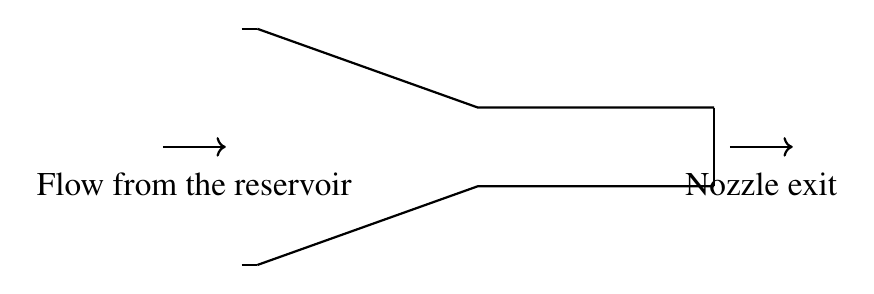
\begin{tikzpicture}
    % Draw the nozzle shape with short vertical lines at the opening
    \draw[thick] (-3,1.5) -- (-2.8,1.5);
    \draw[thick] (-3,-1.5) -- (-2.8,-1.5);
    \draw[thick] (-2.8,1.5) -- (0,0.5) -- (3,0.5);
    \draw[thick] (-2.8,-1.5) -- (0,-0.5) -- (3,-0.5);
    
    % Vertical line at the nozzle exit
    \draw[thick] (3,0.5) -- (3,-0.5);

    % Flow direction arrows
    \draw[->, thick] (-4,0) -- (-3.2,0);
    \draw[->, thick] (3.2,0) -- (4,0);

    % Labels for the flow and nozzle exit, placed below arrows
    \node[below] at (-3.6,-0.2) {\large Flow from the reservoir};
    \node[below] at (3.6,-0.2) {\large Nozzle exit};
\end{tikzpicture}

	\begin{enumerate}
    \item $F=56.389 kN$ and $\theta=28.28\degree$
    \item $F=-56.389 kN$ and $\theta=-28.28\degree$
    \item $F=9.055 kN$ and $\theta=1.414\degree$
    \item $F=-9.055 kN$ and $\theta=-1.414\degree$
\end{enumerate}
\item A particle moves along a curve whose parametric equations are: $x=t^3+2t$, $y=-3e^{-2t}$ and $z=2\sin{5t}$, where $x,\;y$ and $z$ show variations of the distance covered by the particle \brak{\text{in} \;cm} with time $t$ \brak{\text{in}\;s}. The magnitude of the acceleration of the particle  ({in}\;$\frac{cm}{s^2}$) at $t=0$ is $\underline{\hspace{2cm}}$
\item A traffic office imposes on an average $5$ number of penalties  daily on traffic violators. Assume that the number of penalties on different days is independent and follows a Poisson distribution. The probability that there will be less than $4$ penalties in a day is $\underline{\hspace{2cm}}$
\item Mathematical idealization of a crane has three had three bars with their vertices arranged as shown in the figure with a load of $80\;kN$ hanging vertically. The coordinates of the vertices are given in parentheses. The force in the member $QR$, $F_{QR}$ will be 
	%input of figure 2
	\begin{figure}[!ht]
\centering
\resizebox{3cm}{3cm}{%
\begin{circuitikz}
\tikzstyle{every node}=[font=\LARGE]
\draw [ line width=0.6pt](2.75,12) to[sinusoidal voltage source, sources/symbol/rotate=auto] (3.25,11.5);
\draw [ line width=0.6pt](3.25,11.75) to[european resistor] (9.5,11.75);
\draw [line width=0.6pt, ->, >=Stealth] (9.5,11.75) -- (9.5,11);
\draw [ line width=0.6pt](4,12.25) to[short] (4,11.25);
\draw [ line width=0.6pt](4,11.5) to[short] (4,11);
\draw [ line width=0.6pt](8.75,12.25) to[short] (8.75,11);
\draw [ line width=0.6pt](4,11.25) to[short] (4.5,11.25);
\draw [ line width=0.6pt](8.75,11.25) to[short] (8.25,11.25);
\draw [ line width=0.6pt](4.25,11.25) to[short] (5.25,11.25);
\draw [ line width=0.6pt](8.25,11.25) to[short] (7.25,11.25);
\draw [ line width=0.6pt](5,11.25) to[european resistor] (5,8.5);
\draw [ line width=0.6pt](7.5,11.25) to[european resistor] (7.5,8.5);
\draw [ line width=0.6pt](4.75,8.5) to[short] (8,8.5);
\draw [line width=0.6pt, ->, >=Stealth] (6.25,8.5) -- (6.25,7.75);
\node [font=\normalsize] at (6.75,8) {Bus 3};
\node [font=\normalsize] at (4,12.5) {Bus 1};
\node [font=\normalsize] at (8.75,12.5) {Bus 2};
\node [font=\normalsize] at (6.25,12.25) {j q};
\node [font=\normalsize] at (4.5,10) {j r};
\node [font=\normalsize] at (8.25,9.75) {j p};
\end{circuitikz}
}%

\label{fig:my_label}
\end{figure}

\begin{enumerate}
    \item $30\;kN$ Compressive
    \item $30\;kN$ Tensile
    \item $50\;kN$ Compressive
    \item $50\;kN$ Tensile
\end{enumerate}
\item For the cantilever beam of span $3\;m$ \brak{\text{shown below}}, a concentrated load of $20\;kN$ applied at the free end causes a vertical displacement of $2\;mm$ at a section located at a distance of $1\;m$ from the fixed end. If a concentrated vertically downward load of $10\; kN$ is applied at the section located at a distance of $1\;m$ from the fixed end \brak{\text{with no other load on the beam }}, the maximum vertical displacement in the same beam \brak{\text{in} mm} is \underline{\hspace{2cm}}
	%input for figure 3
	\begin{figure}[!ht]
\centering
\resizebox{3cm}{3cm}{%
\begin{circuitikz}
\tikzstyle{every node}=[font=\small]
\draw (4.25,12.25) to[battery1] (4.25,7.75);
\draw (4.25,12.25) to[short] (6.25,12.25);
\draw (4.25,7.75) to[short] (6.25,7.75);
\draw (6.25,12.25) to[R] (6.25,10.25);
\draw (6.25,10.25) to[R] (6.25,7.75);
\draw (6.25,10.25) to[short] (8.75,10.25);
\draw (6.25,7.75) to[short] (8.75,7.75);
\draw (8.75,7.75) to[R] (8.75,9.25);
\draw (8.75,10.25) to[D] (8.75,9);
\node [font=\small] at (4,10.25) {+};
\node [font=\small] at (4,9.75) {-};
\node [font=\small] at (4.75,10.5) {24 Volt};
\node [font=\small] at (6.75,11.25) {12 k$\Omega$};
\node [font=\small] at (6.75,9) {6 k$\Omega$};
\node [font=\small] at (8,8.5) {3.3 k$\Omega$};
\end{circuitikz}
}%

\label{fig:my_label}
\end{figure}

\item For the truss shown below, the member $PQ$ is short by $3\;mm$. The magnitude of vertical displacement of joint $R\brak{\text{in} mm}$ is \underline{\hspace{2cm}}\\
	%input for figure 4
	\begin{figure}[H]
\centering
\resizebox{3cm}{3cm}{%
\begin{circuitikz}
\tikzstyle{every node}=[font=\small]
\draw [->, >=Stealth] (3.5,10.75) -- (3.5,13.75);
\draw [->, >=Stealth] (3.5,10.75) -- (10.75,10.75);
\draw [->, >=Stealth] (2.25,10.75) -- (3.25,10.75);
\draw [dashed] (4.5,13.25) -- (4.5,8.25);
\draw [dashed] (7.25,13.25) -- (7.25,8.25);
\draw [dashed] (10,13.25) -- (10,8.25);
\draw [dashed] (2,8.25) -- (10,8.25);
\draw [dashed] (2,13) -- (10,13);
\draw [short] (4.5,10.75) -- (7.25,11.75);
\draw [short] (7.25,11.75) -- (10,9.75);
\draw [short] (4.5,10.75) -- (10,9.75);
\node [font=\small] at (2.5,11) {$M>1$};
\node [font=\small] at (3.5,14) {$y$};
\node [font=\small] at (11,10.75) {$x$};
\node [font=\small] at (4.5,8) {$X_A$};
\node [font=\small] at (7.25,8) {$X_B$};
\node [font=\small] at (10,8) {$X_C$};
\node [font=\small] at (1.75,8.25) {$Y_{II}$};
\node [font=\small] at (1.75,13) {$Y_I$};
\node [font=\small] at (5.5,11) {$\alpha$};
\node [font=\small] at (6.5,10.5) {$\alpha$};
\node [font=\small] at (9,10) {$2\alpha$};
\end{circuitikz}
}%
\label{fig:my_label}
\end{figure}



\item A rectangular beam of width \brak{b} $230\;mm$ and effective depth \brak{d} $450\;mm$ is reinforced with four bars of $12\;mm$ diameter. The grade of concrete is $M20$ and grade of steel is $Fe500$. Given that for $M20$ grade of concrete the ultimate shear strength, $\tau_{uc}=0.36\;\frac{N}{mm^2}$ for steel percentage, $p=0.25$, and $\tau_{uc}=0.48\;\frac{N}{mm^2}$ for $p=0.50$. For a factored shear force of $45\;kN$, the diameter \brak{\text{in}mm} of $Fe500$ steel two legged stirrups to be used at spacing of $375\;mm$, should be
\begin{enumerate}
    \item $8$
    \item $10$
    \item $12$
    \item $16$
\end{enumerate}
\item The tension and shear force \brak{\text{both in} kN} in the bolt of the joint, as shown below, respectively are
	% input for figure 5
	\begin{figure}[!ht]
\centering
\resizebox{3cm}{3cm}{%
\begin{circuitikz}
\tikzstyle{every node}=[font=\small]
\draw [line width=0.6pt, short] (4,10.75) -- (8.25,10.75);
\draw [line width=0.6pt, short] (8.25,10.75) -- (9.75,12);
\draw [line width=0.6pt, short] (8.25,10.25) -- (9.75,11.5);
\draw [line width=0.6pt, short] (8.25,10.25) -- (9.75,9.25);
\draw [line width=0.6pt, short] (4,9.75) -- (8.25,9.75);
\draw [line width=0.6pt, ->, >=Stealth] (9.75,11.75) -- (10.25,12.25);
\draw [line width=0.6pt, ->, >=Stealth] (9.5,9) -- (10,8.5);
\draw [line width=0.6pt, ->, >=Stealth] (3.75,10.25) -- (5,10.25);
\node [font=\small] at (3.5,10.25) {$Q$};
\node [font=\small] at (10.5,12.5) {$Q_1$};
\node [font=\small] at (10.25,8.25) {$Q_2$};
\draw [line width=0.6pt, short] (8.25,9.75) -- (9.25,9);
\end{circuitikz}
}%

\end{figure}

\begin{enumerate}
    \item $30.33$ and $20.00$
    \item $30.33$ and $25.00$
    \item $33.33$ and $20.00$
    \item $33.33$ and $25.00$
\end{enumerate}
\item For a beam of cross-section, width=$230\;mm$ and effective depth=$500\;mm$, the number of rebars of $12\;mm$ diameter required to satisfy 
minimum tension reinforcement requirement specified by $IS:456-2000$ \brak{\text{assuming grade of steel reinforcement as Fe500}} is \underline{\hspace{2cm}}
\item In a reinforced concrete section, the stress at the extreme fiber in compression is $5.8\;MPa$. The depth of neutral axis in the section is $58\;mm$ and the grade of concrete is $M25$. Assuming linear elastic behavior of the concrete, the effective curvature of the section $\brak{\text{in per}mm} $
\begin{enumerate}
    \item $2.0 \times 10^{-6}$
    \item $3.0 \times 10^{-6}$
    \item $4.0 \times 10^{-6}$
    \item $5.0 \times 10^{-6}$
\end{enumerate}
\item Group $I$ contains representative load-settlement curves for different modes of bearing capacity failures of sandy soil. Group $II$ enlists the various failure characteristics. Match the load-settlement curves with the corresponding failure characteristics.   \\
	%input for figure 6
	\begin{figure}[H]
\centering
\resizebox{3cm}{3cm}{%
\begin{circuitikz}
\tikzstyle{every node}=[font=\large]
\draw [ line width=0.6pt ] (5.5,12.5) rectangle (7.5,6.25);
\draw [line width=0.6pt, dashed] (6.5,12.5) -- (6.5,6.25);
\draw [line width=0.6pt, dashed] (4.75,12.5) -- (8.5,12.5);
\draw [line width=0.6pt, dashed] (4.75,12.75) -- (8.5,12.75);
\draw [line width=0.6pt, dashed] (4.75,13) -- (8.5,13);
\draw [line width=0.6pt, dashed] (4.75,13.25) -- (8.5,13.25);
\draw [line width=0.6pt, dashed] (4.75,13.5) -- (8.5,13.5);
\draw [line width=0.6pt, ->, >=Stealth] (4.5,10.5) -- (4.5,8.75);
\draw [line width=0.6pt, <->, >=Stealth] (8.5,12.5) -- (8.5,6.25);
\node [font=\large] at (4,9.75) {$g$};
\node [font=\large] at (9.25,9.5) {L};
\end{circuitikz}
}%

\label{fig:my_label}
\end{figure}

\begin{tabular}{ll}
    \textbf{Group I} & \textbf{Group II} \\
    \brak{P} Curve $J$          & \brak{i} No apparent heaving of soil around the footing         \\
    \brak{Q} Curve $K$         & \brak{ii} Rankine's passive zone develops imperfectly       \\
    \brak{R} Curve $L$        & \brak{iii} Well defined slip surface extends to ground surface    \\
\end{tabular}

\begin{enumerate}
    \item $P-1,\;Q-3,\;R-2$
    \item $P-3,\;Q-2,\;R-1$
    \item $P-3,\;Q-1,\;R-2$
    \item $P-1,\;Q-2,\;R-3$
\end{enumerate}
\item A given cohesionless soil has $e_{max}=0.85$ and $e_{min}=0.50$. In the field, the soil is compacted to a mass density of $1800\;\frac{kg}{m^3}$ at a water content of $8\%$. Take the mass density of water as $1000\;\frac{kg}{m^3}$ and $G_s$ as $2.7$. The relative density \brak{\text{in}\; \%} of the soil is
\begin{enumerate}
    \item $56.43$
    \item $60.25$
    \item $62.87$
    \item $65.71$
\end{enumerate}
\item The following data are given for the laboratory sample.\\
$\sigma_0'=175\;kPa;\:e_o=1.1;\:\sigma_o'+\Delta \sigma_o'=300\;kPa;\:e=0.9$\\
If the thickness of the clay specimen is $25\;mm$, the value of the coefficient of volume compressibility is \underline{\hspace{2cm}}$\times 10^{-4}\;\frac{m^2}{kN}$

\end{enumerate}
\end{document}
